\section{Gerrymandering} \label{sec:Gerrymandering}

\index{gerrymander}
 \begin{tabular}{m{.45\textwidth}m{.45\textwidth}}
	 The process of dividing the state into the appropriate number of districts is called redistricting, but in the popular press, it is often referred to as gerrymandering.  This is because the map-makers often decide to split things up to their benefit.  One of the earliest, most obvious examples of this was in 1812 when Massachusetts Governor Gerry and his party drew one district in such a curvy and jagged manner that the local press thought it looked like a Salamander (see Figure \ref{fig:gerrymander}) and coined the term Gerrymander. &
%\begin{wrapfigure}{r}{.5\columnwidth}
%\begin{figure}[htb]%
%\caption{The Original Gerrymander}%

\includegraphics[width=.5\columnwidth]{gerrymander}%
\label{fig:gerrymander}%
%\end{figure}
%\end{wrapfigure}
\end{tabular}


Consider the simple state\footnote{Diagrams adapted from Stephen Nass, ``How to Steal an Election''}: 
\newcommand{\district}{
	%locations of participants
	\begin{scope}[shift = {(-.1, -.1)}]
			\draw[very thick] (0,0) -- (10,0) -- (10,5) -- (0,5) -- cycle;
	\end{scope}
	 \foreach \y in {0,1}
	 \foreach \x in {0,1,2,3,4,5,6,7,8,9}
    \draw[teal, opacity = .2, fill = teal] (\x,\y) rectangle (\x+.8,\y+.8);
	 \foreach \y in {2,3,4}
	 \foreach \x in {0,1,2,3,4,5,6,7,8,9}
    \draw[orange, fill=orange] (\x,\y) rectangle (\x+.8,\y+.8);
}

%\begin{wrapfigure}{l}{.5\columnwidth}
\begin{center}
	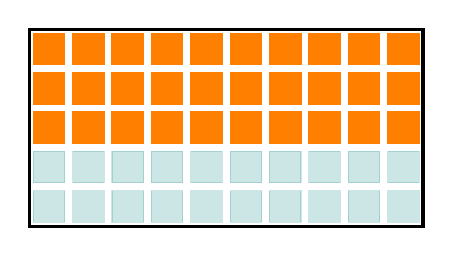
\begin{tikzpicture}[scale=.5]
	\district
\end{tikzpicture}
\end{center}
%\end{wrapfigure}

There are 50 people in this state who belong to two different political parties.  The census says that they should have 5 seats, so we need to divide up these people into 5 groups.  
\begin{enumerate}
	 \begin{tabular}{m{.45\textwidth}m{.45\textwidth}}
	 \item Consider the following districting of this state. Who would win with a majority of votes in each district?  Who has an advantage in the legislature?  Does it seem fair? Are the people in each district connected to each other?  Are the districts generally compact? &\newcommand{\districta}{\begin{scope}[shift = {(-.1,-.1)}]
		\draw[very thick] (0,0 ) -- (10, 0 );
		\draw[very thick] (0,1 ) -- (10, 1 );
		\draw[very thick] (0,2 ) -- (10, 2 );
		\draw[very thick] (0,3 ) -- (10, 3 );
		\draw[very thick] (0,4 ) -- (10, 4 );
		\end{scope}}
	
	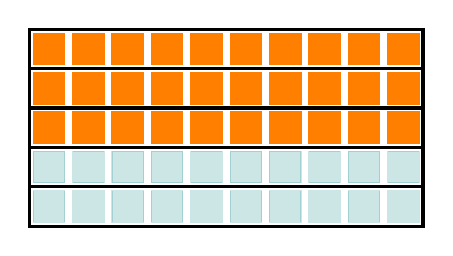
\begin{tikzpicture}[scale=.5]
		\district 
		\begin{scope}[shift = {(-.1,-.1)}]
			\draw[very thick] (0,0 ) -- (10, 0 );
		\draw[very thick] (0,1 ) -- (10, 1 );
		\draw[very thick] (0,2 ) -- (10, 2 );
		\draw[very thick] (0,3 ) -- (10, 3 );
		\draw[very thick] (0,4 ) -- (10, 4 );
		\end{scope}
			\end{tikzpicture} 
	 
	\end{tabular}
	
	
	\vfill
	\clearpage
	 \begin{tabular}{m{.45\textwidth}m{.45\textwidth}}
	 \item Consider the following districting of this state. Who would win with a majority of votes in each district?  Who has an advantage in the legislature?  Does it seem fair? Are the people in each district connected to each other?  Are the districts generally compact? &
	\newcommand{\districtb}{	
	\begin{scope}[shift={(-.1,-.1)}]
					\foreach \x in {0,2,4,6,8}
	\draw[very thick] (\x,0) -- (\x, 5);

	\end{scope}
	}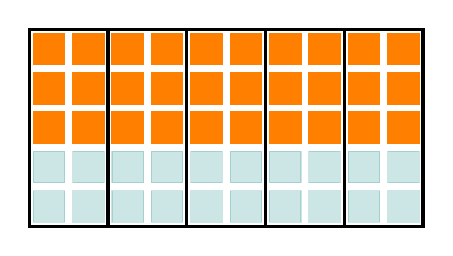
\begin{tikzpicture}[scale=.5]
	\district
	\districtb
	\end{tikzpicture}
	\end{tabular}
	 
	\vfill
 \begin{tabular}{m{.5\textwidth}m{.5\textwidth}}
	 \item Consider the following districting of this state. Who would win with a majority of votes in each district?  Who has an advantage in the legislature?  Does it seem fair? Are the people in each district connected to each other?  Are the districts generally compact? &
		\newcommand{\districtc}{
		\begin{scope}[shift = {(-.1, -.1)}]
				\draw[very thick] (0,0) -- (0,1) -- (1,1) -- (1,4) -- (3,4) -- (3,1) -- (4,1) -- (4,0);
				\draw[very thick] (3,4) -- (4,4) -- (4,2) -- (5, 2) -- (5,5);
				\draw[very thick] (5, 2) -- (6,2) -- (6,4) -- (9,4) -- (9, 1) -- (10, 1);
				\draw[very thick] (7,4) -- (7,1) -- (6,1) -- (6,0);
		\end{scope}
}

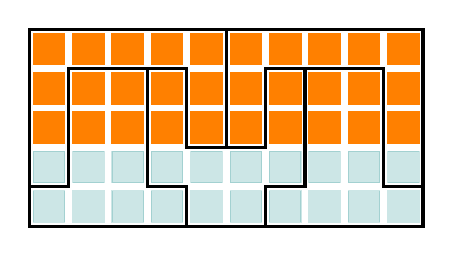
\begin{tikzpicture}[scale=.5]
\district
	\districtc	
	\end{tikzpicture} \end{tabular}
	 
	\vfill

	

The last diagram is an example of the `packing' and `cracking' that are illustrative of modern gerrymandering.
\begin{description}
	\item[packing] Putting a very large number of voters who all vote the same way in a single district.  In this case, the election is won by these voters, but by a very large margin.\index{gerrymander!packing}
	\item[cracking] Putting a slight majority of voters for one party in a single district.  In this case, the election is won by these voters by a slim margin.  There are a lot of minority voters in the district, but not enough to ever win an election.\index{gerrymander!cracking}
\end{description}
\clearpage

\item The state below has approximately 40\% orange (\tikz{\draw[fill=orange,orange]  circle(1ex);}) people and 60\% teal (\tikz{\draw[fill=teal,teal, opacity = .2]  circle(1ex);}) people (each color was selected randomly).  Divide the state into 10 districts in such a way so that in an election 40\% of the seats will be won by the orange people and 60\% by the teal people.

\newcommand{\firstexample}{	\begin{scope}[shift = {(-.9, -.9)}]
\draw[teal, fill = teal, opacity = 0.4] (1, 1) rectangle (1.8, 1.8);	\draw[orange, fill = orange] (1, 2) rectangle (1.8, 2.8);	\draw[orange, fill = orange] (1, 3) rectangle (1.8, 3.8);	\draw[orange, fill = orange] (1, 4) rectangle (1.8, 4.8);	\draw[teal, fill = teal, opacity = 0.4] (1, 5) rectangle (1.8, 5.8);	\draw[orange, fill = orange] (1, 6) rectangle (1.8, 6.8);	\draw[orange, fill = orange] (1, 7) rectangle (1.8, 7.8);	\draw[teal, fill = teal, opacity = 0.4] (1, 8) rectangle (1.8, 8.8);	\draw[orange, fill = orange] (1, 9) rectangle (1.8, 9.8);	\draw[orange, fill = orange] (1, 10) rectangle (1.8, 10.8);
\draw[teal, fill = teal, opacity = 0.4] (2, 1) rectangle (2.8, 1.8);	\draw[teal, fill = teal, opacity = 0.4] (2, 2) rectangle (2.8, 2.8);	\draw[teal, fill = teal, opacity = 0.4] (2, 3) rectangle (2.8, 3.8);	\draw[teal, fill = teal, opacity = 0.4] (2, 4) rectangle (2.8, 4.8);	\draw[teal, fill = teal, opacity = 0.4] (2, 5) rectangle (2.8, 5.8);	\draw[orange, fill = orange] (2, 6) rectangle (2.8, 6.8);	\draw[teal, fill = teal, opacity = 0.4] (2, 7) rectangle (2.8, 7.8);	\draw[orange, fill = orange] (2, 8) rectangle (2.8, 8.8);	\draw[teal, fill = teal, opacity = 0.4] (2, 9) rectangle (2.8, 9.8);	\draw[teal, fill = teal, opacity = 0.4] (2, 10) rectangle (2.8, 10.8);
\draw[teal, fill = teal, opacity = 0.4] (3, 1) rectangle (3.8, 1.8);	\draw[teal, fill = teal, opacity = 0.4] (3, 2) rectangle (3.8, 2.8);	\draw[teal, fill = teal, opacity = 0.4] (3, 3) rectangle (3.8, 3.8);	\draw[teal, fill = teal, opacity = 0.4] (3, 4) rectangle (3.8, 4.8);	\draw[teal, fill = teal, opacity = 0.4] (3, 5) rectangle (3.8, 5.8);	\draw[orange, fill = orange] (3, 6) rectangle (3.8, 6.8);	\draw[orange, fill = orange] (3, 7) rectangle (3.8, 7.8);	\draw[teal, fill = teal, opacity = 0.4] (3, 8) rectangle (3.8, 8.8);	\draw[teal, fill = teal, opacity = 0.4] (3, 9) rectangle (3.8, 9.8);	\draw[teal, fill = teal, opacity = 0.4] (3, 10) rectangle (3.8, 10.8);
\draw[orange, fill = orange] (4, 1) rectangle (4.8, 1.8);	\draw[teal, fill = teal, opacity = 0.4] (4, 2) rectangle (4.8, 2.8);	\draw[teal, fill = teal, opacity = 0.4] (4, 3) rectangle (4.8, 3.8);	\draw[teal, fill = teal, opacity = 0.4] (4, 4) rectangle (4.8, 4.8);	\draw[orange, fill = orange] (4, 5) rectangle (4.8, 5.8);	\draw[orange, fill = orange] (4, 6) rectangle (4.8, 6.8);	\draw[orange, fill = orange] (4, 7) rectangle (4.8, 7.8);	\draw[teal, fill = teal, opacity = 0.4] (4, 8) rectangle (4.8, 8.8);	\draw[teal, fill = teal, opacity = 0.4] (4, 9) rectangle (4.8, 9.8);	\draw[teal, fill = teal, opacity = 0.4] (4, 10) rectangle (4.8, 10.8);
\draw[teal, fill = teal, opacity = 0.4] (5, 1) rectangle (5.8, 1.8);	\draw[orange, fill = orange] (5, 2) rectangle (5.8, 2.8);	\draw[teal, fill = teal, opacity = 0.4] (5, 3) rectangle (5.8, 3.8);	\draw[teal, fill = teal, opacity = 0.4] (5, 4) rectangle (5.8, 4.8);	\draw[orange, fill = orange] (5, 5) rectangle (5.8, 5.8);	\draw[teal, fill = teal, opacity = 0.4] (5, 6) rectangle (5.8, 6.8);	\draw[teal, fill = teal, opacity = 0.4] (5, 7) rectangle (5.8, 7.8);	\draw[teal, fill = teal, opacity = 0.4] (5, 8) rectangle (5.8, 8.8);	\draw[teal, fill = teal, opacity = 0.4] (5, 9) rectangle (5.8, 9.8);	\draw[teal, fill = teal, opacity = 0.4] (5, 10) rectangle (5.8, 10.8);
\draw[orange, fill = orange] (6, 1) rectangle (6.8, 1.8);	\draw[teal, fill = teal, opacity = 0.4] (6, 2) rectangle (6.8, 2.8);	\draw[orange, fill = orange] (6, 3) rectangle (6.8, 3.8);	\draw[teal, fill = teal, opacity = 0.4] (6, 4) rectangle (6.8, 4.8);	\draw[orange, fill = orange] (6, 5) rectangle (6.8, 5.8);	\draw[teal, fill = teal, opacity = 0.4] (6, 6) rectangle (6.8, 6.8);	\draw[orange, fill = orange] (6, 7) rectangle (6.8, 7.8);	\draw[orange, fill = orange] (6, 8) rectangle (6.8, 8.8);	\draw[orange, fill = orange] (6, 9) rectangle (6.8, 9.8);	\draw[orange, fill = orange] (6, 10) rectangle (6.8, 10.8);
\draw[teal, fill = teal, opacity = 0.4] (7, 1) rectangle (7.8, 1.8);	\draw[teal, fill = teal, opacity = 0.4] (7, 2) rectangle (7.8, 2.8);	\draw[teal, fill = teal, opacity = 0.4] (7, 3) rectangle (7.8, 3.8);	\draw[teal, fill = teal, opacity = 0.4] (7, 4) rectangle (7.8, 4.8);	\draw[teal, fill = teal, opacity = 0.4] (7, 5) rectangle (7.8, 5.8);	\draw[teal, fill = teal, opacity = 0.4] (7, 6) rectangle (7.8, 6.8);	\draw[teal, fill = teal, opacity = 0.4] (7, 7) rectangle (7.8, 7.8);	\draw[orange, fill = orange] (7, 8) rectangle (7.8, 8.8);	\draw[orange, fill = orange] (7, 9) rectangle (7.8, 9.8);	\draw[teal, fill = teal, opacity = 0.4] (7, 10) rectangle (7.8, 10.8);
\draw[teal, fill = teal, opacity = 0.4] (8, 1) rectangle (8.8, 1.8);	\draw[orange, fill = orange] (8, 2) rectangle (8.8, 2.8);	\draw[teal, fill = teal, opacity = 0.4] (8, 3) rectangle (8.8, 3.8);	\draw[teal, fill = teal, opacity = 0.4] (8, 4) rectangle (8.8, 4.8);	\draw[teal, fill = teal, opacity = 0.4] (8, 5) rectangle (8.8, 5.8);	\draw[orange, fill = orange] (8, 6) rectangle (8.8, 6.8);	\draw[orange, fill = orange] (8, 7) rectangle (8.8, 7.8);	\draw[orange, fill = orange] (8, 8) rectangle (8.8, 8.8);	\draw[teal, fill = teal, opacity = 0.4] (8, 9) rectangle (8.8, 9.8);	\draw[orange, fill = orange] (8, 10) rectangle (8.8, 10.8);
\draw[teal, fill = teal, opacity = 0.4] (9, 1) rectangle (9.8, 1.8);	\draw[orange, fill = orange] (9, 2) rectangle (9.8, 2.8);	\draw[orange, fill = orange] (9, 3) rectangle (9.8, 3.8);	\draw[teal, fill = teal, opacity = 0.4] (9, 4) rectangle (9.8, 4.8);	\draw[orange, fill = orange] (9, 5) rectangle (9.8, 5.8);	\draw[orange, fill = orange] (9, 6) rectangle (9.8, 6.8);	\draw[teal, fill = teal, opacity = 0.4] (9, 7) rectangle (9.8, 7.8);	\draw[orange, fill = orange] (9, 8) rectangle (9.8, 8.8);	\draw[teal, fill = teal, opacity = 0.4] (9, 9) rectangle (9.8, 9.8);	\draw[teal, fill = teal, opacity = 0.4] (9, 10) rectangle (9.8, 10.8);
\draw[orange, fill = orange] (10, 1) rectangle (10.8, 1.8);	\draw[teal, fill = teal, opacity = 0.4] (10, 2) rectangle (10.8, 2.8);	\draw[teal, fill = teal, opacity = 0.4] (10, 3) rectangle (10.8, 3.8);	\draw[orange, fill = orange] (10, 4) rectangle (10.8, 4.8);	\draw[teal, fill = teal, opacity = 0.4] (10, 5) rectangle (10.8, 5.8);	\draw[teal, fill = teal, opacity = 0.4] (10, 6) rectangle (10.8, 6.8);	\draw[orange, fill = orange] (10, 7) rectangle (10.8, 7.8);	\draw[teal, fill = teal, opacity = 0.4] (10, 8) rectangle (10.8, 8.8);	\draw[teal, fill = teal, opacity = 0.4] (10, 9) rectangle (10.8, 9.8);	\draw[orange, fill = orange] (10, 10) rectangle (10.8, 10.8);

	\end{scope}
}
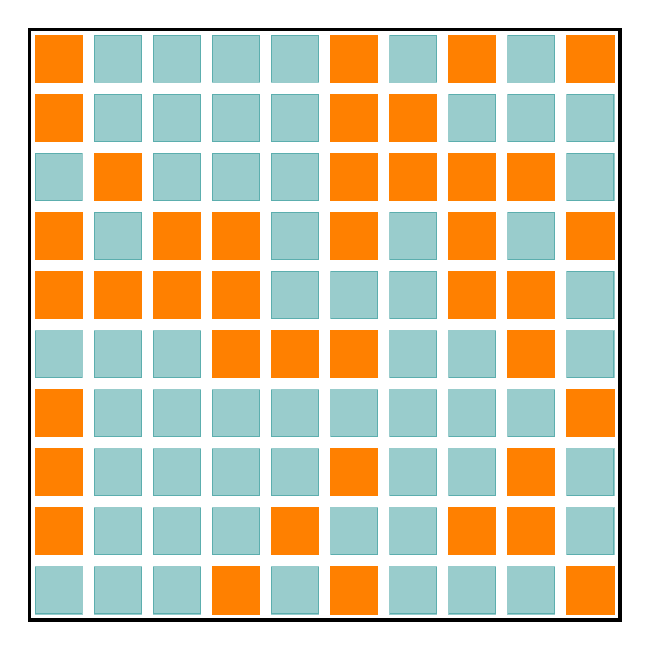
\begin{tikzpicture}[scale=.75]
	\firstexample
	\begin{scope}[]
		\draw[very thick] (0,0) -- (0,10) -- (10,10) -- (10,0) -- cycle;
	\end{scope}
\end{tikzpicture}
\vfill

\item Now, divide the same state in such a way so that 60\% of the seats will be won by the orange people.\\
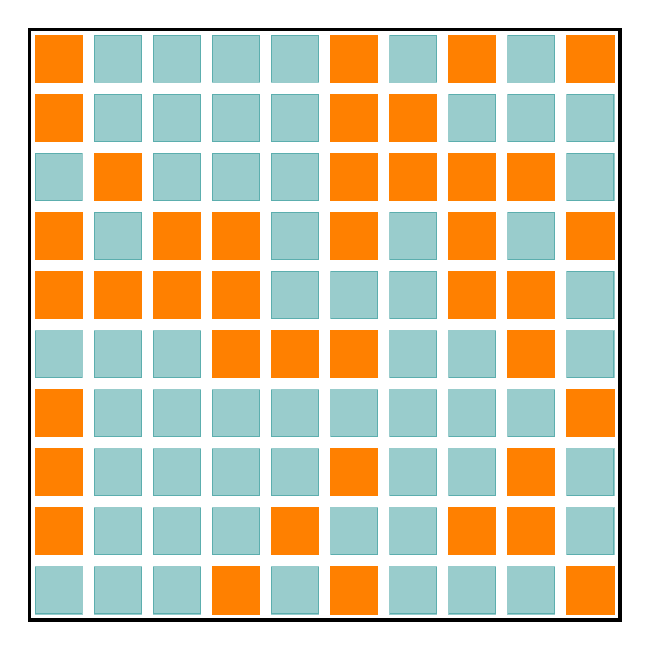
\begin{tikzpicture}[scale = .75]
	\firstexample
	\begin{scope}[]
		\draw[very thick] (0,0) -- (0,10) -- (10,10) -- (10,0) -- cycle;
	\end{scope}
\end{tikzpicture}
\vfill

\end{enumerate}
%<*HWHEADER>
\clearpage
%%%%%%%%%%%%%%%%%%%%%%%%%%%%%%%%%%%%%%%%%%%%%%%%%%%%%%%%%%%%%%%%%%%%%%%%%%%%%%%%%%%%%%%%%%%%%%%%%%%%%%%%
\HOMEWORK
%</HWHEADER>

%<*HOMEWORK>


\begin{Renumerate}

  \item Consider the following map.  Put 5 districts on the map so that orange receives the most seats.
	\newcommand{\homeworkone}{
		\begin{scope}[shift = {(-.9,-.9)}]
			\draw[orange, fill = orange] (1, 1) rectangle (1.8, 1.8);	
			\draw[teal, fill = teal, opacity = 0.4] (1, 2) rectangle (1.8, 2.8);	
			\draw[teal, fill = teal, opacity = 0.4] (1, 3) rectangle (1.8, 3.8);	
			\draw[teal, fill = teal, opacity = 0.4] (1, 4) rectangle (1.8, 4.8);	
			\draw[orange, fill = orange] (1, 5) rectangle (1.8, 5.8);
			\draw[orange, fill = orange] (2, 1) rectangle (2.8, 1.8);	
			\draw[teal, fill = teal, opacity = 0.4] (2, 2) rectangle (2.8, 2.8);	
			\draw[teal, fill = teal, opacity = 0.4] (2, 3) rectangle (2.8, 3.8);	
			\draw[teal, fill = teal, opacity = 0.4] (2, 4) rectangle (2.8, 4.8);	
			\draw[teal, fill = teal, opacity = 0.4] (2, 5) rectangle (2.8, 5.8);
			\draw[teal, fill = teal, opacity = 0.4] (3, 1) rectangle (3.8, 1.8);	
			\draw[orange, fill = orange] (3, 2) rectangle (3.8, 2.8);	
			\draw[teal, fill = teal, opacity = 0.4] (3, 3) rectangle (3.8, 3.8);	
			\draw[teal, fill = teal, opacity = 0.4] (3, 4) rectangle (3.8, 4.8);	
			\draw[teal, fill = teal, opacity = 0.4] (3, 5) rectangle (3.8, 5.8);
			\draw[orange, fill = orange] (4, 1) rectangle (4.8, 1.8);	
			\draw[orange, fill = orange] (4, 2) rectangle (4.8, 2.8);	
			\draw[orange, fill = orange] (4, 3) rectangle (4.8, 3.8);	
			\draw[orange, fill = orange] (4, 4) rectangle (4.8, 4.8);	
			\draw[teal, fill = teal, opacity = 0.4] (4, 5) rectangle (4.8, 5.8);
			\draw[teal, fill = teal, opacity = 0.4] (5, 1) rectangle (5.8, 1.8);	
			\draw[teal, fill = teal, opacity = 0.4] (5, 2) rectangle (5.8, 2.8);	
			\draw[orange, fill = orange] (5, 3) rectangle (5.8, 3.8);	
			\draw[teal, fill = teal, opacity = 0.4] (5, 4) rectangle (5.8, 4.8);	
			\draw[orange, fill = orange] (5, 5) rectangle (5.8, 5.8);
	\end{scope}
}
	
\begin{center}
		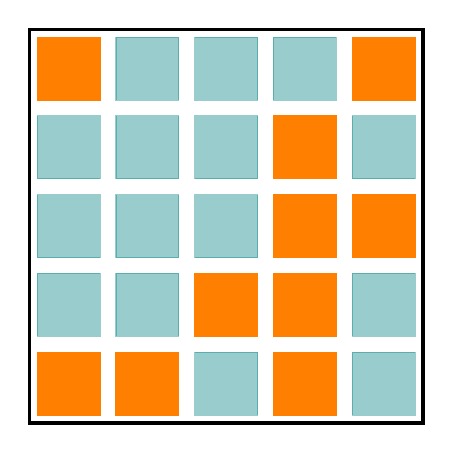
\begin{tikzpicture}
		\homeworkone
		\begin{scope}
			\draw[very thick] (0,0) -- (0,5) -- (5,5) -- (5,0)  --cycle;
		\end{scope}
	\end{tikzpicture}

\end{center}	
	\item Put 5 districts on the map so that teal receives the most districts.
	
\begin{center}
			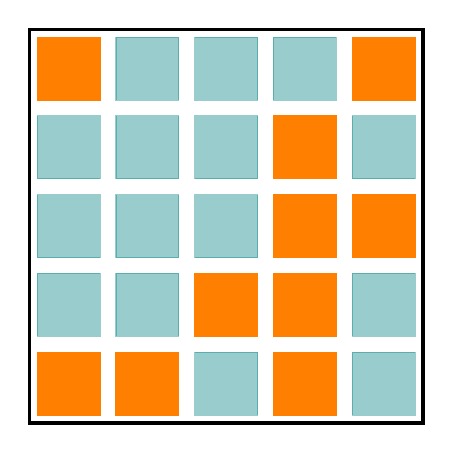
\begin{tikzpicture}
		\homeworkone
		
		\begin{scope}
			\draw[very thick] (0,0) -- (0,5) -- (5,5) -- (5,0)  --cycle;
		\end{scope}
	\end{tikzpicture}

\end{center}
\end{Renumerate} 

\ENDHOMEWORK

%%%%%%%%%%%%%%%%%%%%%%%%%%%%%%%%%%%%%%%%%%%%%%%%%%%%%%%%%%%%%%%%%%%%%%%%%%%%%%%%%%%%%%%%%%%%%

\clearpage
